\chapter{Plano de atividades para o próximo período}\label{chp:plano}

As últimas realizações foram bem acompanhadas por pesquisas novas referências e aprofundamento matemático do problema de calibração encontrado. Ademais, o assunto de calibração é um tema estudado próximo ao anos 2000 e não é discutido atualmente em forma de artigos, mas, em contrapartida, foram encontrados referências na documentação do \textit{OpenCV} e vídeo-aulas como a de Pavel, desenvolvidas na Seção \ref{chp:biblio}. Como um reflexo desse estudo, e a continuação da implementação apresentada na Seção \ref{chp:impl}, definimos um objetivo sólido de prosseguir com a programação da calibração e finalizar as duas etapas (extrínseca e intrínseca) da calibração da projeção em realidade aumentada.

\begin{figure}[H]
   \centering
   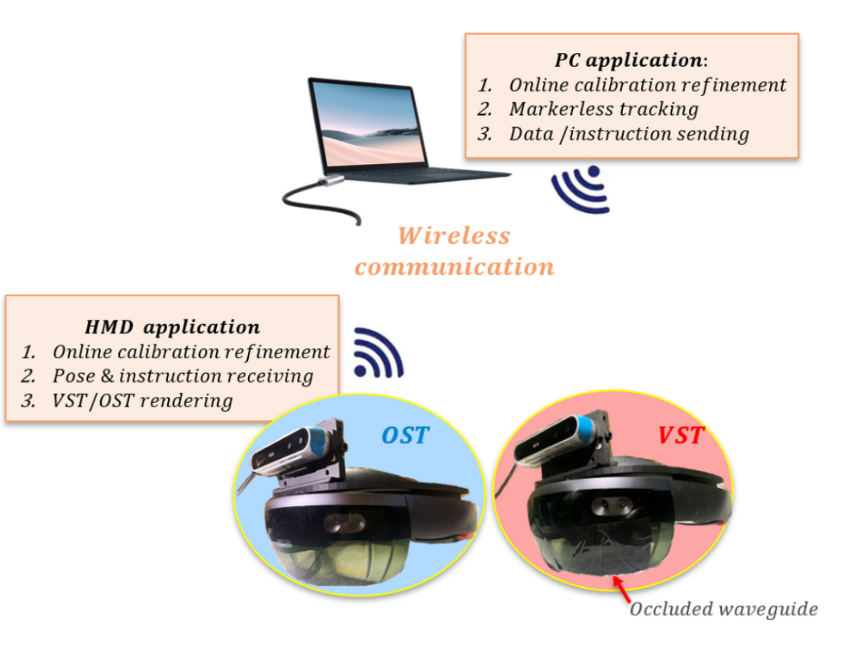
\includegraphics[width=.7\linewidth]{figuras/cutoloSys.png}
   \caption{Arquitetura de sistema recentemente publicado. Utiliza conexão sem fio e um \textit{Microsoft Hololens 1} para funcionamento em \textit{OST} e \textit{VST}. Fonte: \cite{Hu2022}}
   \label{fig:cutolo}
\end{figure}

Durante a revisão bibliográfica, foi encontrado um artigo que desenvolve um sistema que auxilia cirurgias ortopédicas utilizando AR. Neste, foram apresentados dois tipos de projeção em realidade aumentada: \textit{VST} ou \textit{video see-through} consiste em exibir um vídeo com a projeção; e \textit{OST} ou \textit{optical see-through} funciona projetando a imagem da sobreposição em um \textit{display} semi-transparente \cite{Hu2022}. 

Ambos os tipos de projeção podem ser feitos com o \textit{Moverio BT-350}, porém, a quantidade de materiais de estudo disponíveis para o \textit{VST} são muito maiores pois é o tipo de projeção mais popular e presente em \textit{smartphones}, \textit{tablets} e óculos de realidade virtual. Por conta disso, foi decidido implementar primeiramente o sistema em \textit{VST}, mesmo os nossos equipamentos permitindo o \textit{OST}. Dessa forma, temos uma maior versatilidade utilizar o \textit{VCranium} também em outros dispositivos além de óculos de realidade aumentada.

\begin{figure}[H]
   \centering
   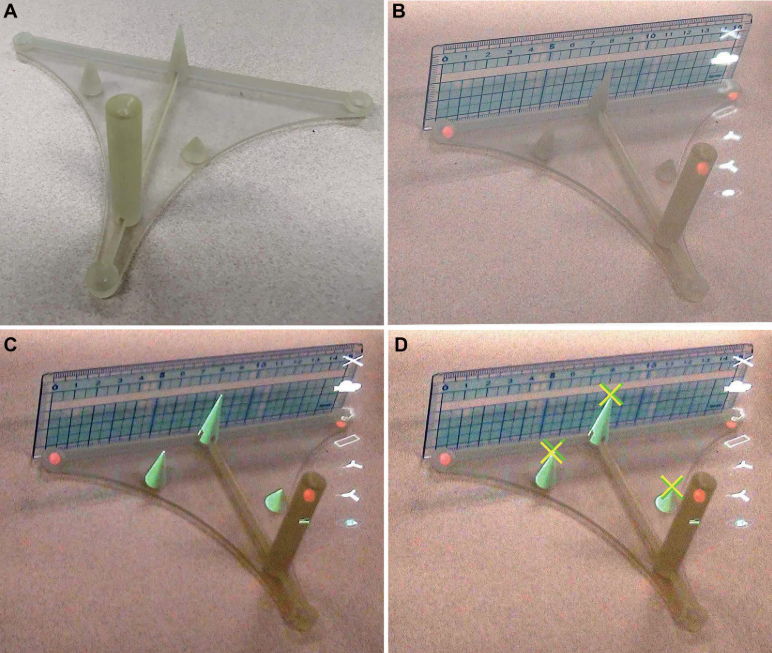
\includegraphics[width=.65\linewidth]{figuras/phantom.png}
   \caption{A figura demonstra a construção a utilização do calibrador (\textit{phantom}) para a medição do erro da projeção em realidade aumentada. Fonte: \cite{Maruyama2018}}
   \label{fig:phantom}
\end{figure}

Após finalizarmos a calibração da projeção, temos que utilizar um método para medir a sua precisão. Esse campo já foi estudado no artigo de Maruyama, onde foi necessário construir um modelo calibrador que serve como alvo para o algoritmo calcular o erro da visualização, observável na Figura \ref{fig:phantom}. Portanto, a tarefa final do projeto é escolher um método de verificação de erro após a pesquisa e a listagem dos métodos possíveis.